\documentclass[a4paper, 10pt]{article}

\usepackage[T2A]{fontenc}
\usepackage[utf8]{inputenc}
\usepackage[english, russian]{babel}
\usepackage[top=2cm, bottom=2cm, right=2cm, left=2cm]{geometry}
\usepackage{amsmath}
\usepackage{graphicx}
\usepackage{subcaption}
\usepackage{float}
\usepackage{tabularx}

\usepackage{amsmath,booktabs}
\usepackage{array}

\usepackage{tabu}
\newcommand\tline[2]{$\underset{\text{#1}}{\text{\underline{\hspace{#2}}}}$}
%Change label separator
\usepackage{caption}
\captionsetup[figure]{name = Рисунок, labelsep = endash}
\captionsetup[table]{labelformat=simple, labelsep = endash, justification = raggedright, singlelinecheck = off, width = 0.9\textwidth}

\usepackage{indentfirst}
\usepackage{setspace}
% одинарный интервал
\singlespacing
% полуторный интервал
\onehalfspacing
% двойной интервал
\doublespacing
% произвольный интервал
\setstretch{1}

\begin{document}
	\parindent=1.27cm
	\begin{titlepage}
		\centering
		{\fontsize{12pt}{5cm}\selectfont \bfseries Министерство образования и науки Российской Федерации} \\ \vspace{0.5cm}
		{\fontsize{7pt}{5cm}\selectfont ФЕДЕРАЛЬНОЕ ГОСУДАРСТВЕННОЕ АВТОНОМНОЕ ОБРАЗОВАТЕЛЬНОЕ УЧРЕЖДЕНИЕ ВЫСШЕГО ПРОФЕССИОНАЛЬНОГО ОБРАЗОВАНИЯ} \\ 
		\vspace{1cm}
		{\fontsize{12pt}{5cm}\selectfont \bfseries САНКТ-ПЕТЕРБУРГСКИЙ УНИВЕРСИТЕТ ИНФОРМАЦИОННЫХ ТЕХНОЛОГИЙ, МЕХАНИКИ И ОПТИКИ} \\ \vspace{1.5cm}

		{\fontsize{14pt}{5cm}\selectfont Кафедра \hspace{1cm} \underline{Систем Управления и Информатики}  \hspace{1cm} Группа \underline{Р3340}} \\ 
		\vspace{2cm}

		{\fontsize{20pt}{5cm}\selectfont \bfseries Лабораторная работа №7} \\
		{\fontsize{20pt}{5cm}\selectfont \bfseries “Анализ точности систем управления”} \\
		{\fontsize{14pt}{5cm}\selectfont Вариант - 11} \\
		\vspace{1.5cm}

		\flushleft

		{Выполнил \hspace{2cm} \tline{(фамилия, и.о.)}{9cm} (подпись)} \\
		\vspace{2cm}

		{Проверил \hspace{2cm} \tline{(фамилия, и.о.)}{9cm} (подпись)} \\
		\vspace{5cm}

		"\underline{\hspace{0.7cm}}"\hspace{0.2cm}\underline{\hspace{2cm}}\hspace{0.2cm}20\underline{\hspace{0.7cm}}г. \hspace{2cm} Санкт-Петербург, \hspace{2cm} 20\underline{\hspace{0.7cm}}г. \\ \vspace{1cm}

		Работа выполнена с оценкой \hspace{1cm} \underline{\hspace{8cm}} \\ 
		\vspace{1cm}
		Дата защиты "\underline{\hspace{0.7cm}}"\hspace{0.2cm}\underline{\hspace{2cm}}\hspace{0.2cm}20\underline{\hspace{0.7cm}}г.

\end{titlepage}

\paragraph{Цель работы: }Исследование точностных свойств систем управления.
\paragraph{Исходные данные} Ниже в таблице 1 представленны параметры системы и возмущающих воздействий.

\begin{table} [h!]
	\centering
	\caption{Исходные данные.}
	\tabulinesep = 2mm
	\begin{tabu} spread 1em{|c|c|c|c|c|c|c|c|}
		\hline
		$W(s)$ & $g = A$ & $g = Vt$ & $g = at^2/2$ & Вариант схемы & $f_1$ & $f_2$ & Сигнал задания \\  \hline
		$\aligned \frac{1}{0.5s^{2} +s + 1} \endaligned$ & 2 & 2t & $0.45t^2$ &  г) & -0.5 & 0,25 & $0.3t + 2\sin{(0.8t)}$ \rule{0pt}{5pt} \\ 
		\hline
	\end{tabu}
\end{table}
\clearpage
\begin{center}
\section{Исследование системы с астатизмом нулевого порядка}\hfill\par
\end{center}
Задана замкнутая система с регулятором $H(s)=k$ и передаточной функцией разомкнутого контура 
\begin{equation}
W(s) = \frac{1}{{0.5{s^2} + s + 1}}
\end{equation}

\begin{figure}[h]
	\centering
	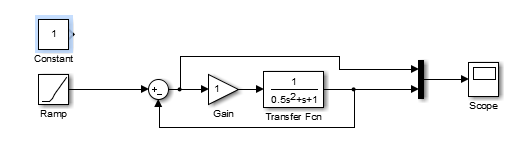
\includegraphics[width=0.7\linewidth]{12}
	\caption{Схема моделирования}
	\label{fig:12}
\end{figure}

\subsection{Исследование стационарного режима работы при g(t)=2}\hfill\par
Рассчитаем предельное значение установившейся ошибки

\begin{equation}
\varepsilon  = \frac{1}{{1 + H\left( s \right)W\left( s \right)}}G\left( s \right) = \mathop {\lim }\limits_{s \to 0} s\frac{1}{{1 + \frac{k}{{0.5{s^2} + s + 1}}}}\frac{2}{s} = \mathop {\lim }\limits_{s \to 0} \frac{{{s^2} + 2s + 2}}{{0.5{s^2} + s + 1 + k}} = \frac{2}{{1 + k}}
\end{equation}

таким образом, найдём ощибки для различных значений $k$:
$\varepsilon=1 (k=1), \varepsilon=0.33 (k=5), \varepsilon=0.18 (k=10)$

\begin{center}
	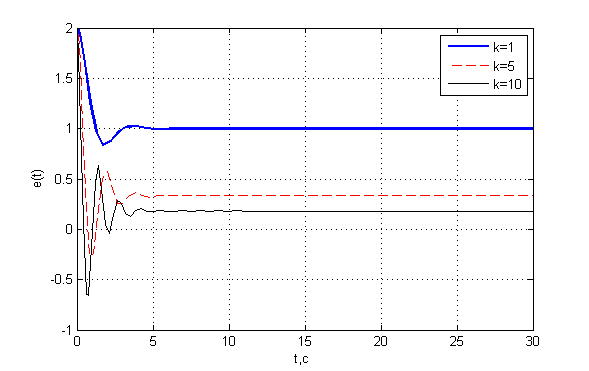
\includegraphics[width=0.7\linewidth]{1}
	\begin{figure}[ht]
	
	\caption{Графика ошибки е(t)}
	\label{fig:1}
	\end{figure}
\end{center}

\begin{figure}[h]
	\centering
	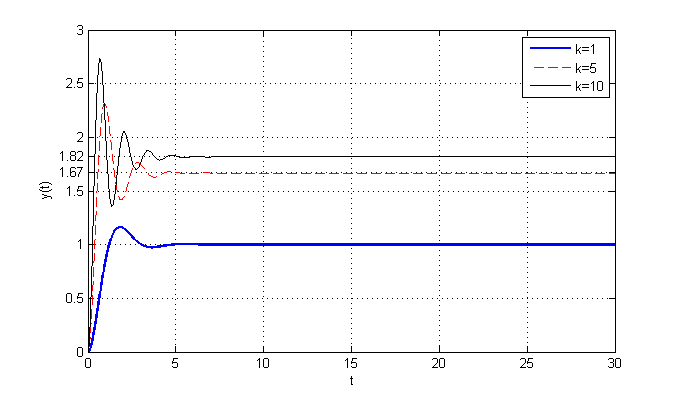
\includegraphics[width=0.7\linewidth]{2}
	\caption{Графика переходных процессов}
	\label{fig:2}
\end{figure}

\subsection{Исследование режима движения с постоянной скоростью при g(t)=2t}\hfill\par
Рассчитаем предельное значение установившейся ошибки\\
\begin{equation}
\varepsilon  = \frac{1}{{1 + H\left( s \right)W\left( s \right)}}G\left( s \right) = \mathop {\lim }\limits_{s \to 0} s\frac{1}{{1 + \frac{k}{{0.5{s^2} + s + 1}}}}\frac{2}{{{s^2}}} = \mathop {\lim }\limits_{s \to 0} \frac{{0.5{s^2} + s + 1}}{{0.5{s^2} + s + 1 + k}}\frac{2}{s} = \infty 
\end{equation}
\begin{center}

	\begin{figure}[h]
		\centering
			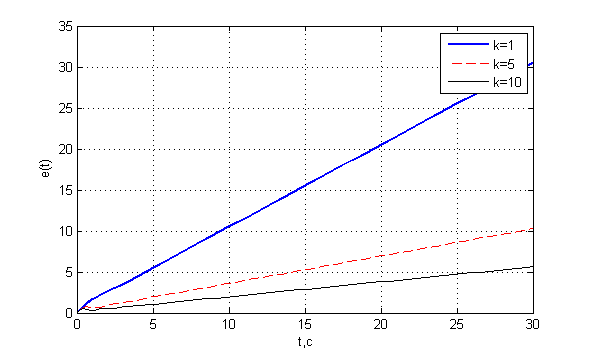
\includegraphics[width=0.7\linewidth]{33}
		\caption{Графика ошибки е(t)}
		\label{fig:33}
	\end{figure}
\end{center}

\begin{figure}[H]
	\centering
	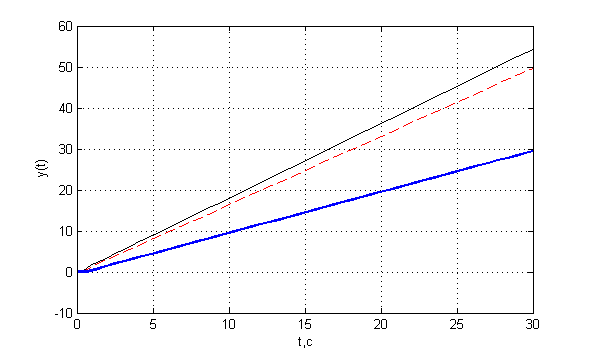
\includegraphics[width=0.7\linewidth]{44}
	\caption{Графика переходных процессов}
	\label{fig:44}
\end{figure}
\clearpage
\begin{center}
\section{Исследование системы с астатизмом первого порядка.}\hfill\par
\end{center}		
	\begin{figure}[h]
	\center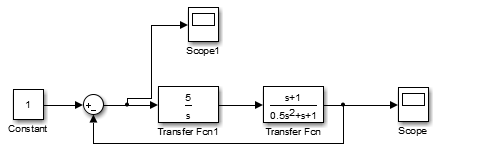
\includegraphics[width=0.6\linewidth]{5}
		\caption{Схема моделирования}
		\label{fig:5}
	\end{figure}

\subsection{Исследование стационарного режима работы при g(t)=2}\hfill\par
Рассчитаем предельное значение установившейся ошибки

\begin{equation}
{e_y}(t) = \mathop {\lim }\limits_{s \to 0} s\frac{1}{{1 + W(s)}}\frac{A}{s} = \mathop {\lim }\limits_{s \to 0} \frac{1}{{1 + \frac{{{W^*}(s)}}{s}}}A = \mathop {\lim }\limits_{x \to 0} \frac{s}{{s + k}}A = 0
\end{equation}

	\begin{figure}[h]
		\centering
		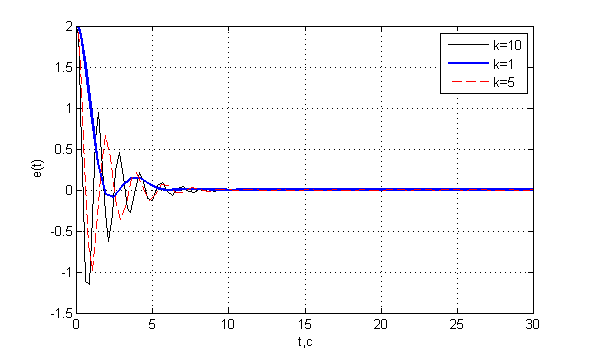
\includegraphics[width=0.7\linewidth]{7}
		\caption{Графика ошибки е(t)}
		\label{fig:7}
	\end{figure}

\subsection{Исследование режима движения с постоянной скоростью при g(t)=2t}\hfill\par
Рассчитаем предельное значение установившейся ошибки
\begin{equation}
\varepsilon  = \mathop {\lim }\limits_{s \to 0} s\frac{1}{{1 + W(s)}}\frac{V}{{{s^2}}} = \mathop {\lim }\limits_{s \to 0} \frac{s}{{s + k}}\frac{V}{s} = \frac{V}{k}
\end{equation}



\begin{center}
	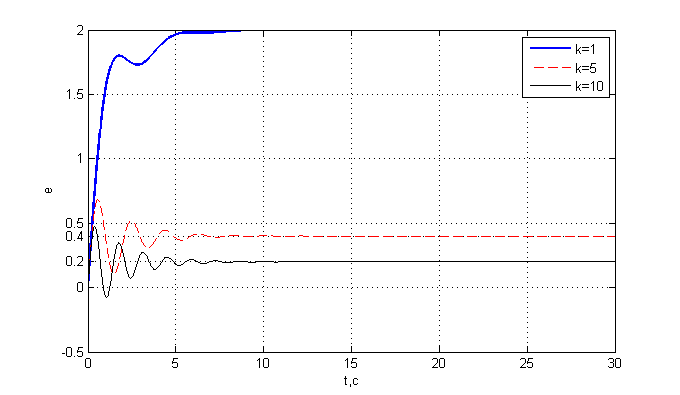
\includegraphics[width=0.7\linewidth]{6}
	\begin{figure}[h]
		\centering
		
		\caption{Графика ошибки е(t)}
		\label{fig:6}
	\end{figure}
\end{center}

таким образом, найдём ощибки для различных значений $k$:
$\varepsilon=2 (k=1), \varepsilon=0.4 (k=5), \varepsilon=0.2 (k=10)$

\subsection{Исследование режима движения с постоянным ускорением g(t)=at}\hfill\par

Рассчитаем предельное значение установившейся ошибки
\begin{equation}
\varepsilon  = \mathop {\lim }\limits_{s \to 0} s\frac{1}{{1 + W(s)}}\frac{a}{{{s^3}}} = \mathop {\lim }\limits_{s \to 0} \frac{s}{{s + k}}\frac{a}{{{s^2}}} = \infty
\end{equation}

\begin{center}
	\begin{figure}[h]
		\centering
		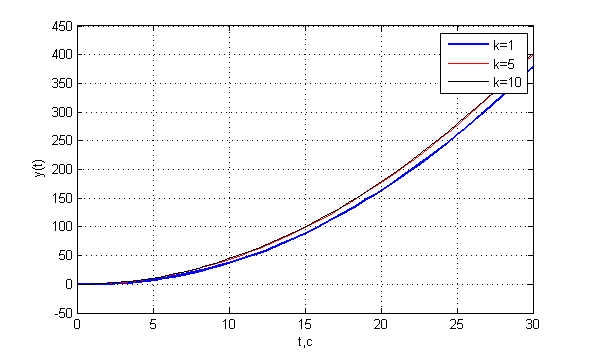
\includegraphics[width=0.7\linewidth]{8}
		\caption{Графика переходных процессов }
		\label{fig:8}
	\end{figure}
\end{center}
\clearpage
\begin{center}
	\section{Исследование влияния внешних возмущений}\hfill\par
\end{center}
\begin{figure}[h]
	\centering
	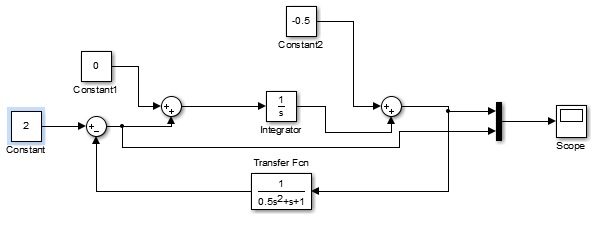
\includegraphics[width=0.7\linewidth]{9}
	\caption{Схема моделирования}
	\label{fig:9}
\end{figure}
Рассчитаем предельное значение установившейся ошибки:
\begin{equation}
\varepsilon  = \mathop {\lim }\limits_{s \to 0} [ - s\frac{{sW(s)}}{{s + W(s)}}\frac{{{F_1}}}{s} + s\frac{{W(s)}}{{s + W(s)}}\frac{{{F_2}}}{s}] = {F_2}
\end{equation}
\begin{center}
	\begin{figure}[H]
		\centering
			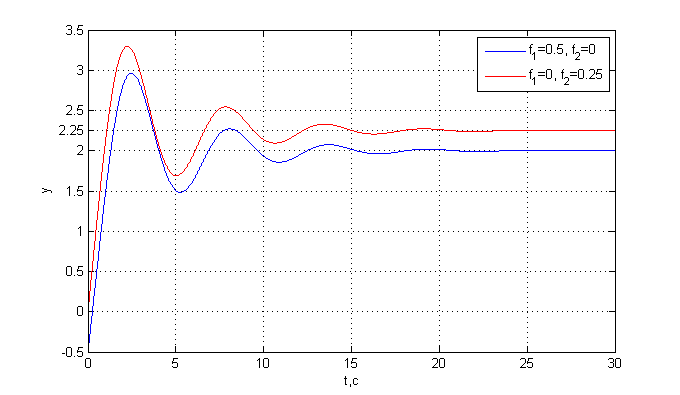
\includegraphics[width=0.7\linewidth]{10}
		\caption{Графика переходных процессов}
		\label{fig:10}
	\end{figure}
\end{center}
\newpage
\begin{figure}[h]
	\centering
	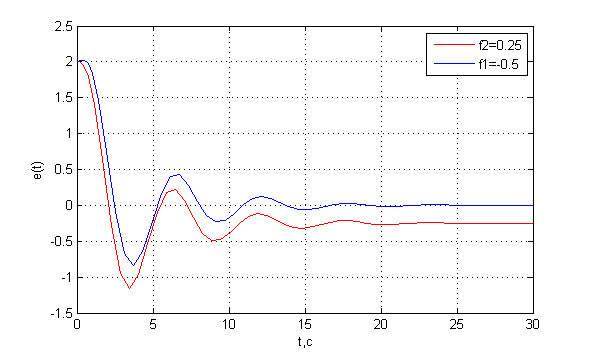
\includegraphics[width=0.7\linewidth]{13}
	\caption{Графика ошибки е(t)}
	\label{fig:13}
\end{figure}
\clearpage
\begin{center}
\section{Исследование установившейся ошибки при произвольном входном воздействии}\hfill\par
\end{center}
\begin{center}
	\begin{figure}[h]
		\centering
	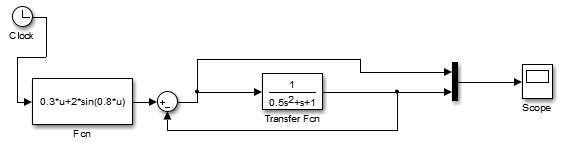
\includegraphics[width=0.7\linewidth]{14}
		\caption{Схема моделирования}
		\label{fig:14}
	\end{figure}
\end{center}

\begin{figure}[h]
	\centering
	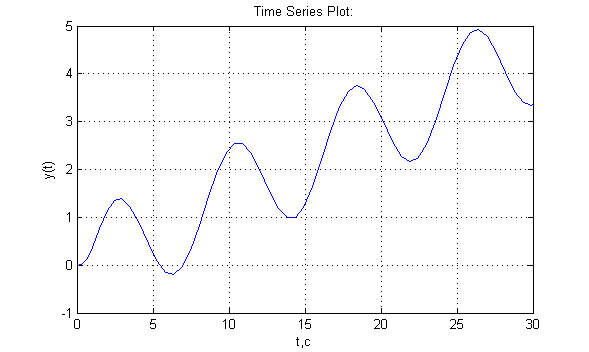
\includegraphics[width=0.7\linewidth]{15}
	\caption{Графика переходного процесса}
	\label{fig:15}
\end{figure}

Оценим приближенно установившуюся ошибку слежения:

\begin{equation}
\varPhi(s) = \frac{1}{{1 + H(s)W(s)}} = \frac{{0.5{s^2} + s + 1}}{{0.5{s^2} + s + 2}}
\end{equation}
Разложим $\varPhi(s)$ в ряд Тейлора в окрестности точки s=0:
% MathType!MTEF!2!1!+-
% feaagGart1ev2aaatCvAUfeBSjuyZL2yd9gzLbvyNv2CaerbuLwBLn
% hiov2DGi1BTfMBaeXatLxBI9gBaerbd9wDYLwzYbItLDharqqtubsr
% 4rNCHbGeaGqiVu0Je9sqqrpepC0xbbL8F4rqqrFfpeea0xe9Lq-Jc9
% vqaqpepm0xbba9pwe9Q8fs0-yqaqpepae9pg0FirpepeKkFr0xfr-x
% fr-xb9adbaqaaeGaciGaaiaabeqaamaabaabaaGcbaGaam4yamaaBa
% aaleaacaaIWaaabeaakiabg2da9maalaaabaGaaGymaaqaaiaaikda
% aaGaeyypa0JaaGimaiaac6cacaaI1aaaaa!3D8B!
\[{c_0} = \frac{1}{2} = 0.5\]
% MathType!MTEF!2!1!+-
% feaagGart1ev2aaatCvAUfeBSjuyZL2yd9gzLbvyNv2CaerbuLwBLn
% hiov2DGi1BTfMBaeXatLxBI9gBaerbd9wDYLwzYbItLDharqqtubsr
% 4rNCHbGeaGqiVu0Je9sqqrpepC0xbbL8F4rqqrFfpeea0xe9Lq-Jc9
% vqaqpepm0xbba9pwe9Q8fs0-yqaqpepae9pg0FirpepeKkFr0xfr-x
% fr-xb9adbaqaaeGaciGaaiaabeqaamaabaabaaGcbaGaam4yamaaBa
% aaleaacaaIXaaabeaakiabg2da9maalaaabaGaamizaaqaaiaadsga
% caWGZbaaaiabfA6agnaaBaaaleaacaWGLbaabeaakiaacIcacaWGZb
% Gaaiykaiabg2da9maalaaabaGaaiikaiaadohacqGHRaWkcaaIXaGa
% aiykaiaacIcacaaIWaGaaiOlaiaaiwdacaWGZbWaaWbaaSqabeaaca
% aIYaaaaOGaey4kaSIaam4CaiabgUcaRiaaikdacaGGPaGaeyOeI0Ia
% aiikaiaaicdacaGGUaGaaGynaiaadohadaahaaWcbeqaaiaaikdaaa
% GccqGHRaWkcaWGZbGaey4kaSIaaGymaiaacMcacaGGOaGaai4Caiab
% gUcaRiaaigdacaGGPaaabaGaaiikaiaaicdacaGGUaGaaGynaiaado
% hadaahaaWcbeqaaiaaikdaaaGccqGHRaWkcaWGZbGaey4kaSIaaGOm
% aiaacMcadaahaaWcbeqaaiaaikdaaaaaaOGaeyypa0ZaaSaaaeaaca
% WGZbGaey4kaSIaaGymaaqaaiaacIcacaaIWaGaaiOlaiaaiwdacaWG
% ZbWaaWbaaSqabeaacaaIYaaaaOGaey4kaSIaam4CaiabgUcaRiaaik
% dacaGGPaWaaWbaaSqabeaacaaIYaaaaaaakiaacYhadaWgaaWcbaGa
% am4Caiabg2da9iaaicdaaeqaaOGaeyypa0ZaaSaaaeaacaaIXaaaba
% GaaGinaaaacqGH9aqpcaaIWaGaaiOlaiaaikdacaaI1aaaaa!7E0D!
\[{c_1} = \frac{d}{{ds}}{\Phi _e}(s) = \frac{{(s + 1)(0.5{s^2} + s + 2) - (0.5{s^2} + s + 1)(s + 1)}}{{{{(0.5{s^2} + s + 2)}^2}}} = \frac{{s + 1}}{{{{(0.5{s^2} + s + 2)}^2}}}{|_{s = 0}} = \frac{1}{4} = 0.25\]
% MathType!MTEF!2!1!+-
% feaagGart1ev2aaatCvAUfeBSjuyZL2yd9gzLbvyNv2CaerbuLwBLn
% hiov2DGi1BTfMBaeXatLxBI9gBaerbd9wDYLwzYbItLDharqqtubsr
% 4rNCHbGeaGqiVu0Je9sqqrpepC0xbbL8F4rqqrFfpeea0xe9Lq-Jc9
% vqaqpepm0xbba9pwe9Q8fs0-yqaqpepae9pg0FirpepeKkFr0xfr-x
% fr-xb9adbaqaaeGaciGaaiaabeqaamaabaabaaGcbaGaam4yamaaBa
% aaleaacaaIYaaabeaakiabg2da9maalaaabaGaamizamaaCaaaleqa
% baGaaGOmaaaaaOqaaiaadsgacaWGZbWaaWbaaSqabeaacaaIYaaaaa
% aakiabfA6agnaaBaaaleaacaWGLbaabeaakiaacIcacaWGZbGaaiyk
% aiabg2da9maalaaabaGaaiikaiaaicdacaGGUaGaaGynaiaadohada
% ahaaWcbeqaaiaaikdaaaGccqGHRaWkcaWGZbGaey4kaSIaaGOmaiaa
% cMcadaahaaWcbeqaaiaaikdaaaGccqGHsislcaGGOaGaam4CaiabgU
% caRiaaigdacaGGPaGaaGOmaiaacIcacaaIWaGaaiOlaiaaiwdacaWG
% ZbWaaWbaaSqabeaacaaIYaaaaOGaey4kaSIaam4CaiabgUcaRiaaik
% dacaGGPaGaaiikaiaadohacqGHRaWkcaaIXaGaaiykaaqaaiaacIca
% caaIWaGaaiOlaiaaiwdacaWGZbWaaWbaaSqabeaacaaIYaaaaOGaey
% 4kaSIaam4CaiabgUcaRiaaikdacaGGPaWaaWbaaSqabeaacaaI0aaa
% aaaakiaacYhadaWgaaWcbaGaam4Caiabg2da9iaaicdaaeqaaOGaey
% ypa0ZaaSaaaeaacaaIYaWaaWbaaSqabeaacaaIYaaaaOGaeyOeI0Ia
% aGOmaiaacQcacaaIYaGaaiOkaiaaigdaaeaacaaIYaWaaWbaaSqabe
% aacaaI0aaaaaaakiabg2da9iaaicdaaaa!7858!
\[{c_2} = \frac{{{d^2}}}{{d{s^2}}}{\Phi _e}(s) = \frac{{{{(0.5{s^2} + s + 2)}^2} - (s + 1)2(0.5{s^2} + s + 2)(s + 1)}}{{{{(0.5{s^2} + s + 2)}^4}}}{|_{s = 0}} = \frac{{{2^2} - 2*2*1}}{{{2^4}}} = 0\]
% MathType!MTEF!2!1!+-
% feaagGart1ev2aaatCvAUfeBSjuyZL2yd9gzLbvyNv2CaerbuLwBLn
% hiov2DGi1BTfMBaeXatLxBI9gBaerbd9wDYLwzYbItLDharqqtubsr
% 4rNCHbGeaGqiVu0Je9sqqrpepC0xbbL8F4rqqrFfpeea0xe9Lq-Jc9
% vqaqpepm0xbba9pwe9Q8fs0-yqaqpepae9pg0FirpepeKkFr0xfr-x
% fr-xb9adbaqaaeGaciGaaiaabeqaamaabaabaaGcbaGaamyzamaaBa
% aaleaacaWG5baabeaakiaacIcacaWG0bGaaiykaiabg2da9iaaicda
% caGGUaGaaGynaiaacIcacaaIWaGaaiOlaiaaiodacaWG0bGaey4kaS
% IaaGOmaiGacohacaGGPbGaaiOBaiaaicdacaGGUaGaaGioaiaacsha
% caGGPaGaey4kaSIaaGimaiaac6cacaaIYaGaaGynaiaacIcacaaIWa
% GaaiOlaiaaiodacqGHRaWkcaaIXaGaaiOlaiaaiAdaciGGJbGaai4B
% aiaacohacaaIWaGaaiOlaiaaiIdacaWG0bGaaiykaiabgkHiTiaaic
% dacqGH9aqpcaaIWaGaaiOlaiaaigdacaaI1aGaaiiDaiabgUcaRiGa
% cohacaGGPbGaaiOBaiaaicdacaGGUaGaaGioaiaadshacqGHRaWkca
% aIWaGaaiOlaiaaisdaciGGJbGaai4BaiaacohacaaIWaGaaiOlaiaa
% iIdacaWG0bGaey4kaSIaaGimaiaac6cacaaIWaGaaG4naiaaiwdaaa
% a!74FB!
\[{e_y}(t) = 0.5(0.3t + 2\sin 0.8t) + 0.25(0.3 + 1.6\cos 0.8t) - 0 = 0.15t + \sin 0.8t + 0.4\cos 0.8t + 0.075\]
\newpage
\begin{figure}[h]
	\centering
	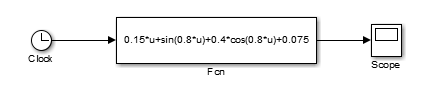
\includegraphics[width=0.7\linewidth]{16}
	\caption{Схема моделирования}
	\label{fig:16}
\end{figure}

\begin{center}
	\begin{figure}[ht]
		\centering
			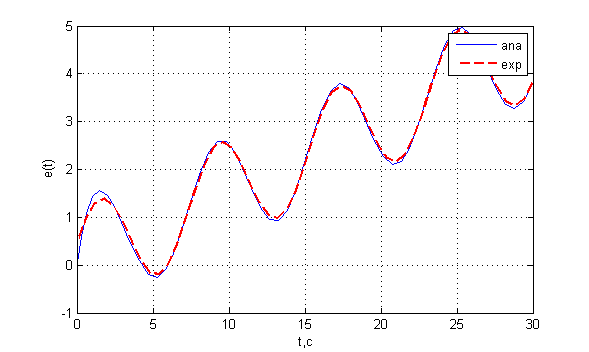
\includegraphics[width=0.7\linewidth]{17}
		\caption{Графика экспериментальной и аналитически вычисленной ощибок е(t)}
		\label{fig:17}
	\end{figure}
\end{center}
\clearpage
\begin{center}
	\section*{Выводы}
\end{center}

В данной работе мы исследовали системы с разными порядками астатизма и различными входными и возмущающими воздействиями. В частности, системы с астатизмом первого порядка нечувствительны к постоянным возмущениям.При исследовании стационарного режима работы, убедились в том, что при g = A, и увеличении коэффициента усиления k ошибка стремиться к нулю. 
Убедились в том, что при увеличении прядка астатизма, ошибка, при статическом входном возвдействии ошибка равна нулю.
Внешние возмущения могут оказвать довольно сильное влияние - изменение выходного сигнала в 2 раза, сильное перерегулироване.
\end{document}
